\documentclass[10pt]{beamer}

\usepackage[utf8]{inputenc}
\usepackage[T1]{fontenc}
\usepackage[french]{babel}
\usepackage[ddmmyyyy]{datetime}
\usepackage{listings,lstautogobble,graphicx,tikz,verbatim, amsthm,amsfonts,amsmath,amssymb,mathrsfs,thmtools}
\usetikzlibrary{arrows,automata}
\usetikzlibrary{positioning}

\usetheme{Warsaw}
\useinnertheme{rectangles}
\setbeamerfont{headline}{size=\large}
\setbeamerfont{frametitle}{size=\normalsize}


%Plan/Sommaire automatique avant chaque section
\AtBeginSection[]{
  \begin{frame}
  \frametitle{Plan}
  \tableofcontents[currentsection]
  \end{frame}
}
\AtBeginSubsection[]
{
    \begin{frame}{Plan}
        \tableofcontents[currentsection,currentsubsection]
    \end{frame}
}

\author{Sonny Klotz - Idir Hamad - Younes Benyamna - Malek Zemni}
\institute{UVSQ}
\date{\today}
\usepackage[french,frenchkw,ruled,vlined]{../texLib/algorithm2e}
\usepackage{../texLib/myInfolines}
\usepackage{longtable,array}
\title{Présentation : projet primalité}

\declaretheorem[name=Théorème]{Th}
\declaretheorem[name=Définition]{Def}

\begin{document}

	\begin{frame}
		\titlepage
	\end{frame}
	
	\section*{Introduction}
	
		\begin{frame}
			Projet de M1 informatique UVSQ sur les tests de primalité :\\~\\
			\begin{itemize}
				\item Existence de plusieurs tests de primalité.
				\item Utilisés pour générer des nombres premiers.
				\item Performances différentes.
			\end{itemize}~\\
			\pause
			\textbf{Objectif :} implémentation, description (rapport) et mesures de performances pour construire un générateur optimal.\\
		\end{frame}
	
		\begin{frame}
			\tableofcontents
		\end{frame}
		
	\section{Architecture}
	
		\begin{frame}
		
		Principales fonctionnalités de l'application développée :\\~\\
			\begin{itemize}
				\item Implémentation de tests de primalité :
					\begin{enumerate}
					\item Test Naif
					\item Test de Wilson
					\item Test de Fermat
					\item Test de Miller-Rabin
					\item Test de Solovay-Strassen
					\item Test AKS
					\end{enumerate}
				\item Mesures de performances.
				\item Génération de nombres premiers.
			\end{itemize}~\\
			
		\end{frame}
		\begin{frame}
		Organigramme de l'application et données échangées :\\
			\begin{center}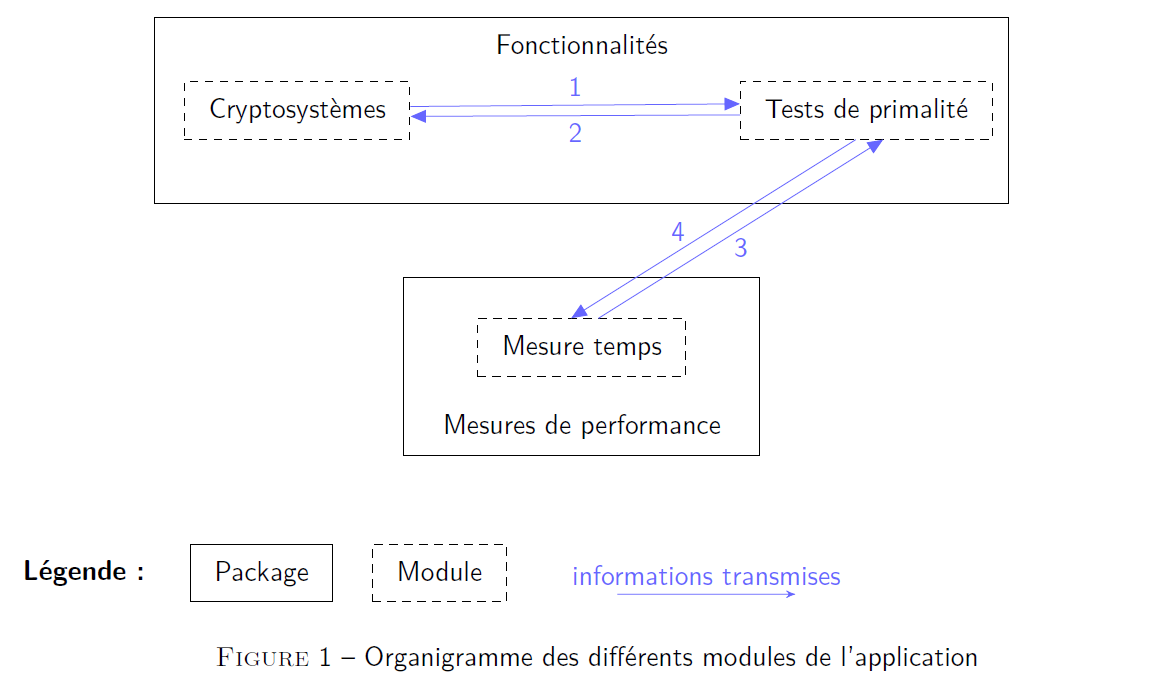
\includegraphics[scale=0.45]{img/org.png}\end{center}
		\end{frame}
		\begin{frame}
		Fonctionnement de l'application :\\~\\
			\begin{itemize}
				\item Mesures de performance de chaque test.
				\item Exploitation des résultats de mesures pour construire le générateur optimal.
				\item Utilisation du générateur par l'utilisateur.
			\end{itemize}
		~\\~\\
		\pause
		Technologies utilisées :\\~\\
			\begin{itemize}
				\item Langage C + GMP
				\item LaTeX
				\item Gnuplot
			\end{itemize}
		\end{frame}
		
	\section{Primalité - cryptosystèmes}
	
		\begin{frame}
			Tests de primalité importants dans la \textbf{cryptographie à clé publique}.\\
			Utilisés pour générer de grands nombres premiers.\\~\\
			\begin{itemize}
			\item \textbf{RSA} : phase de génération des clés.
			\item \textbf{ElGamal} : phase d'échange de clés.
			\end{itemize}
		\end{frame}
		
		\begin{frame}
			Cas de RSA :\\~\\
			\begin{itemize}
			\item Générer 2 grands nombres premiers distincts $p$ et $q$.
			\item Module RSA : $n = p*q$. La taille en bits de $p$ et $q$ est la moitié de celle de $n$.
			\item Calcul de $\phi(n) = (p-1)*(q-1)$.
			\item Clé publique : $e$ premier avec $\phi(n)$.
			\item Clé privée : $d = e^{-1}\pmod\phi(n)$.
			\end{itemize}
			~\\
			Importance des nombres premiers : la \textbf{factorisation} de $n$ permet de retrouver la clé privée $d$.
		\end{frame}
		
	\section{Génération des nombres premiers}
		
		\begin{frame}
			Processus de génération des nombres premiers :\\
			\begin{center}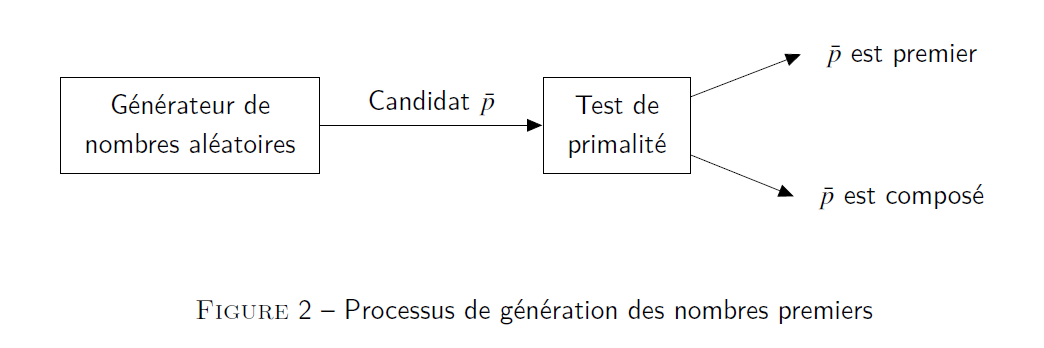
\includegraphics[scale=0.5]{img/gen.png}\end{center}
		\end{frame}
		
		\begin{frame}
			Importance du générateur :\\~\\
			\begin{itemize}
				\item Utilisé par les cryptosystèmes pour générer des nombres premiers.
				\item Importance pour la sécurité : générateur aléatoire imprévisible. 
			\end{itemize}
			~\\
			\pause
			Importance du test de primalité:\\~\\
			\begin{itemize}
				\item Assure que le nombre aléatoire est premier.
				\item Performances du générateur dépend du choix du test de primalité.
			\end{itemize}
		\end{frame}
		
	\section{Tests de primalité}
		\begin{frame}
			Teste si un nombre est \textbf{premier} ou \textbf{composé}.\\~\\
			Existence de plusieurs tests, avec deux type différents :\\
			\begin{itemize}
				\item \textbf{Tests déterministes :} renvoient toujours le bon résultat.
				\item \textbf{Tests probabilistes :} renvoient un résultat avec une certaine probabilité.
			\end{itemize}
			~\\
			\pause
			\begin{table}[H]\begin{center}
				\begin{tabular}{|c|c|c|}
				\hline
				Algorithme           & Année & Type       \\ \hline
				Naïf (Crible d’Eratosthène) & -240  & Déterministe \\ \hline
				Fermat               & 1640  & Probabiliste \\ \hline
				Wilson               & 1770  & Déterministe \\ \hline
				Miller-Rabin         & 1976  & Probabiliste \\ \hline
				Solovay-Strassen     & 1977  & Probabiliste \\ \hline
				AKS                  & 2002  & Déterministe \\ \hline
				\end{tabular}
			\end{center}\end{table}
			
		\end{frame}
		
		\subsection{Test Naïf}
			\begin{frame}
				Méthode la plus intuitive de tester si un nombre est premier ou composé, à laquelle on a effectué plusieurs optimisations :\\~\\
				\begin{center}
				\begin{algorithm}[H]
					\caption{Test naïf}\label{TN}
					\Donnees{un entier $n$}
					\Pour{tout nombre premier $p \leqslant \sqrt{n}$}{
						\Si {$p$ divise $n$}
							{\Retour composé\;}
					}
				\Retour premier\;
				\end{algorithm}
				\end{center}
				~\\
				\textbf{Complexité :} $O(\sqrt{n})$ opérations.
			\end{frame}
		
			\begin{frame}
				Utilisation du \textbf{crible d’Eratosthène} (III\up{e} siècle av. J.-C.) pour pré-calculer et stoker dans une table tous les nombres premiers $\leqslant \sqrt{n}$ :\\~\\
				\begin{center}
					\begin{algorithm}[H]
					\caption{Crible d'Eratosthène}\label{Eras}
					\Donnees{un entier $N$ qui correspond à $\sqrt{n}$}
					{Créer une liste L de couples \textit{(entier, primalité)}, pour les entiers allant de $2$ jusqu'à $N$, avec une primalité initialisée à "premier" : \textit{\textbf{L = \{(2, premier), (3, premier), ..., ($N$, premier)\}}} \;}
					{\textit{\textbf{plusGrandPremier}} = $N$ \;}
					\Pour{tout nombre $p$ marqué "premier" de la liste L (de manière croissante)}{
						\Si{$p^{2}$ > \textit{\textbf{plusGrandPremier}}}{ 
							\Retour L\;
						}
						{\textit{\textbf{i}} = $2$ \;}
						\Tq{$p*i < N$}{ 
							{Marquer "composé" l'entier à la position $p*i$ \;}
							{Mettre à jour \textit{\textbf{plusGrandPremier}} \;}
							{$i++$ \;}
						}
					}
				\end{algorithm}	
				\end{center}
			\end{frame}
			
		\subsection{Test de Wilson}
			\begin{frame}
				Test basé sur une propriété simple : \\~\\
				\begin{center}
				\begin{Th}[Théorème de Wilson]
					Un entier $n > 1$ est un nombre premier si et seulement si
					\[(n-1)! + 1 \equiv 0 \pmod n\]
				\end{Th}
				\end{center}
			\end{frame}
			
			\begin{frame}
				\begin{center}
				\begin{algorithm}[H]
					\caption{Test de Wilson}\label{Wil}
					\Donnees{un entier $n$}
					\Si{$(n-1)! + 1 \equiv 0 \pmod n$} { 
						{\Retour premier\;}
					} \Sinon{
						{\Retour composé\;}
					}
				\end{algorithm}	
				\end{center}
				~\\
				\textbf{Complexité :} $O(n)$.
			\end{frame}
			
		\subsection{Test de Fermat}
			\begin{frame}
				Test de primalité probabiliste basé sur le petit théorème de Fermat :
				\begin{center}
				\begin{Th}[Petit théorème de Fermat (énoncé 1)]
					\label{ThFermat1}
					Si $p$ est un nombre premier, alors pour tout nombre entier $a$ premier avec $p$
					\[a^{p-1}\equiv 1 \pmod p\]
				\end{Th}
				\end{center}
				~\\
				Énoncé la première fois en 1640 par \textit{Pierre de Fermat}.
			\end{frame}
			
			\begin{frame}
				\begin{itemize}
				\item Choix de $1 < a < n$.
				\item Calcul de $\mathbf{a^{n-1} \pmod n}$.
				\item $k$ répétitions.
				\end{itemize}
				\begin{center}
				\begin{algorithm}[H]
					\caption{Test de Fermat}\label{TF}
					\Donnees{un entier $n$ et le nombre de répétitions $k$}
					\Pour{$i$ = $1$ jusqu'à $k$}{
						Choisir aléatoirement $a$ tel que $1 < a < n$\;
						\Si {$a^{n-1} \not\equiv 1 \pmod n$}
							{\Retour composé\;}
					}
				\Retour probablement premier\;
				\end{algorithm}
				\end{center}
			\end{frame}
			
			\begin{frame}
				Présence de nombres \textbf{pseudo-premiers} et nombres de \textbf{Carmichael}.\\~\\
				\begin{Def}[Nombre pseudo-premier]
					\label{PseudoPrem}
					Un nombre pseudo-premier est un nombre premier probable (un entier naturel qui partage une propriété commune à tous les nombres premiers) qui n'est en fait pas premier. Un nombre pseudo-premier provenant du théorème de Fermat est appelé nombre pseudo-premier de Fermat.
				\end{Def}
				~\\
				\begin{Def}[Nombre de Carmichael]
					\label{Carmich}
					Un entier positif composé $n$ est appelé nombre de Carmichael si pour tout entier $a$ premier avec $n$,
					\[a^{n-1}\equiv 1 \pmod n\]
				\end{Def}
			\end{frame}
			
			\begin{frame}
				\textbf{Complexité :} dépend de \\~\\
				\begin{itemize}
				\item la multiplication modulaire : $C_{mult}(n)$
				\item l'exponentiation modulaire \textbf{\textit{Square And Multiply}} : $log_{2}(n) \cdot C_{mult}(n)$
				\end{itemize}
				~\\
				$\Longrightarrow$ Complexité test de Fermat : $O(k \cdot log_{2}(n) \cdot C_{mult}(n))$.
			\end{frame}
		
		\subsection{Test de Miller-Rabin}
			\begin{frame}
			Probabiliste, initialement publié en 1976, basé sur un raffinement du petit théorème de Fermat.\\~\\
			\begin{itemize}
				\item Écriture $\mathbf{n - 1 = 2^{s}t}$ pour $n>0$ et $t$ impair
				\item Exploitation dans la propriété du petit théorème de Fermat : $a^{n-1}\equiv 1 \pmod n$
				\item Établissement de la propriété de primalité, si :
				\[ a^{2^{j}t} \equiv 1 \pmod n \quad \text{pour un } j \in \{0, 1, ..., s-1\} \text{,}\]
				alors $n$ est composé.
			\end{itemize}
			\end{frame}
			
			\begin{frame}
			
				\begin{algorithm}[H]
				\caption{Test de Miller-Rabin}\label{TMR}
				\Donnees{un entier $n$ et le nombre de répétitions $k$}
				{Décomposer $n - 1 = 2^{s}t$, avec $s \in \mathbb{N}^{*}$ et $t \in \mathbb{N}$ impair \;}
				\Pour{$i$ = $1$ jusqu'à $k$}{
					{Choisir aléatoirement $a$ tel que $1 < a < n$\;}
					{$y \gets a^{t} \pmod n$\;}
					\Si{$y \not\equiv 1 \pmod n$ et $y \not\equiv -1 \pmod n$}{
						\Pour{$j = 1$ jusqu'à $s - 1$}{
							{$y \gets y^{2} \pmod n$\;}
							\Si{$y \equiv 1 \pmod n$}{
								{\Retour composé\;}
							}
							\Si{$y \equiv -1 \pmod n$}{
								{Arrêter la boucle de $j$ et continuer avec le $i$ suivant (sans renvoyer composé)\;}
							}
							{\Retour composé\;}
						}
					}
				}
				\Retour probablement premier\;
				\end{algorithm}
		
			\end{frame}
			
			\begin{frame}
				\textbf{Répétitions et probabilité d'erreurs :} la probabilité que le test renvoie premier à tort après $k$ itérations est de $1/4^{k}$.\\~\\
		
				\textbf{Complexité :} $log_{2}(n - 1)$.
			\end{frame}
		
		\subsection{Test de Solovay-Strassen}	
			\begin{frame}
			Probabiliste, publié en 1977, basé sur le \textit{\textbf{critère d'Euler}}.\\~\\
			\begin{Th}[Critère d'Euler]
			\label{CritereEuler}
			Soient $p > 2$ un nombre premier et $a$ un entier premier avec $p$
			\begin{itemize}
				\item Si $a$ est un résidu quadratique modulo $p$, alors $a^{\frac{n-1}{2}} \equiv 1 \pmod p$.
				\item Si $a$ n'est pas un résidu quadratique modulo $p$, alors $a^{\frac{n-1}{2}} \equiv -1 \pmod p$.
			\end{itemize}
			Ceci se résume en utilisant le symbole de Legendre par :
			\[a^{\frac{n-1}{2}} \equiv \left ( \frac{a}{p} \right ) \pmod p\]
			\end{Th}
		
			\end{frame}
			
			\begin{frame}
			\begin{algorithm}[H]
				\caption{Test de Solovay-Strassen}\label{TSS}
				\Donnees{un entier $n$ \underline{impair} et le nombre de répétitions $k$}
				\Pour{$i$ = $1$ jusqu'à $k$}{
					Choisir aléatoirement $a$ tel que $2 < a < n$\;
					$x \gets \left ( \frac{a}{n} \right )$\;
					\Si {$x = 0$ ou $x \not\equiv a^{\frac{n-1}{2}} \pmod n$}{
						{\Retour composé\;}
					}
				}
			\Retour probablement premier\;
			\end{algorithm}
		
			\end{frame}
			
			\begin{frame}
			
			\end{frame}	
		
		\subsection{Test AKS}	
			\begin{frame}
			Déterministe, publié en 2002, temps polynomial, basé sur une généralisation du petit théorème de Fermat :\\~\\
			\begin{Th}[Petit théorème de Fermat généralisé]
			\label{ThFermat4}
			Pour tout entier $n \geqslant 2$ et $a \in \mathbb{Z}$ premiers entre eux,
			\[n \text{  est premier} \quad \Leftrightarrow \quad (X + a)^{n} \equiv X^{n} + a \pmod n\] 
			Le symbole $X$ représente un symbole formel.
			\end{Th}
			\end{frame}
			
			\begin{frame}
			\begin{algorithm}[H]
				\caption{Test AKS}\label{AKS}
				\Donnees{un entier $n > 1$}
				
				1 - \Si {$n = a^{b}$ pour des entiers $a > 1$ et $b > 1$}{\Retour composé\;}
				
				2 - Déterminer le plus petit entier $r$ tel que $Ord_{r}(n) > log_{2}(n)^{2}$ dans $\mathbb{Z}_{r}$ (si $r$ n'est pas premier avec $n$, on passe cet $r$)\;
				
				3 - \Pour {tout $a \leq r$}{
						\Si{$1 < pgcd(a,n) < n$}{
							\Retour composé\;
						}
					}
				
				4 - \Si {$n \leq r$}{\Retour premier\;}
				
				5 - \Pour{$a = 1$ jusqu'à $\lfloor\sqrt{\varphi(r)} log_{2}(n)\rfloor{}{}$}{
						\Si {$(X + a)^{n} \quad \not\equiv \quad X^{n} + a\quad$ dans $ \frac{\mathbb{Z}/n\mathbb{Z}[X]}{ (X^{r} - 1)\mathbb{Z}/n\mathbb{Z}[X]}$}{
							\Retour composé\;
					}
				}
				6 - \Retour premier\;
			\end{algorithm}
			\end{frame}
			
			\begin{frame}
				\textbf{Complexité :}
			\end{frame}	
		
	\section{Comparatifs - Performances}	
		\begin{frame}
			\textbf{Évolution des tests de primalité :}\\~\\
			\pause
			\begin{itemize}
			\item Premiers tests déterministes
				\begin{itemize}
				\item Test Naïf - Crible d'Eratosthène (III\up siècle avant J-C.)
				\item Test de Wilson (1770)
				\end{itemize}
			\pause
			\item Tests probabilistes
				\begin{itemize}
				\item Test de Fermat (1640) longuement utilisé
				\item Apparition du test de Solovay-Strassen (1977)
				\item Remplacés par le test de Miller-Rabin à partir de 1980 (bonne probabilité)
				\end{itemize}
			\pause
			\item Test déterministe rapide : AKS (2002), complexité polynomiale, améliorations envisageables
			\end{itemize}
		\end{frame}
		
		\begin{frame}
			\textbf{Mesures de performance : temps d'exécution}\\~\\
			\begin{algorithm}[H]
				\caption{Mesure temps exécution}\label{MEST}
				\Donnees{tableau tps[6][1025] à remplir, correspondant au temps d'exécution des 6 test pour un nombre de bits entre 0 et 1024}
				\Sortie{tableau tps[6][1025] rempli}
				\Pour{chaque test ($i$ = $0$ jusqu'à $5$)}{
					\Pour{pour un nombre de bits allant de 0 à 1024 ($j$ = $0$ jusqu'à $1024$)}{
						Générer un nombre premier $p$ de $j$ bits\;
						tps[i][j] $\gets$ temps pour que le test $i$ vérifie $p$\;
					}
				}
			\end{algorithm}
		\end{frame}
		
		\begin{frame}
			\begin{figure}[H]\makebox[\textwidth]{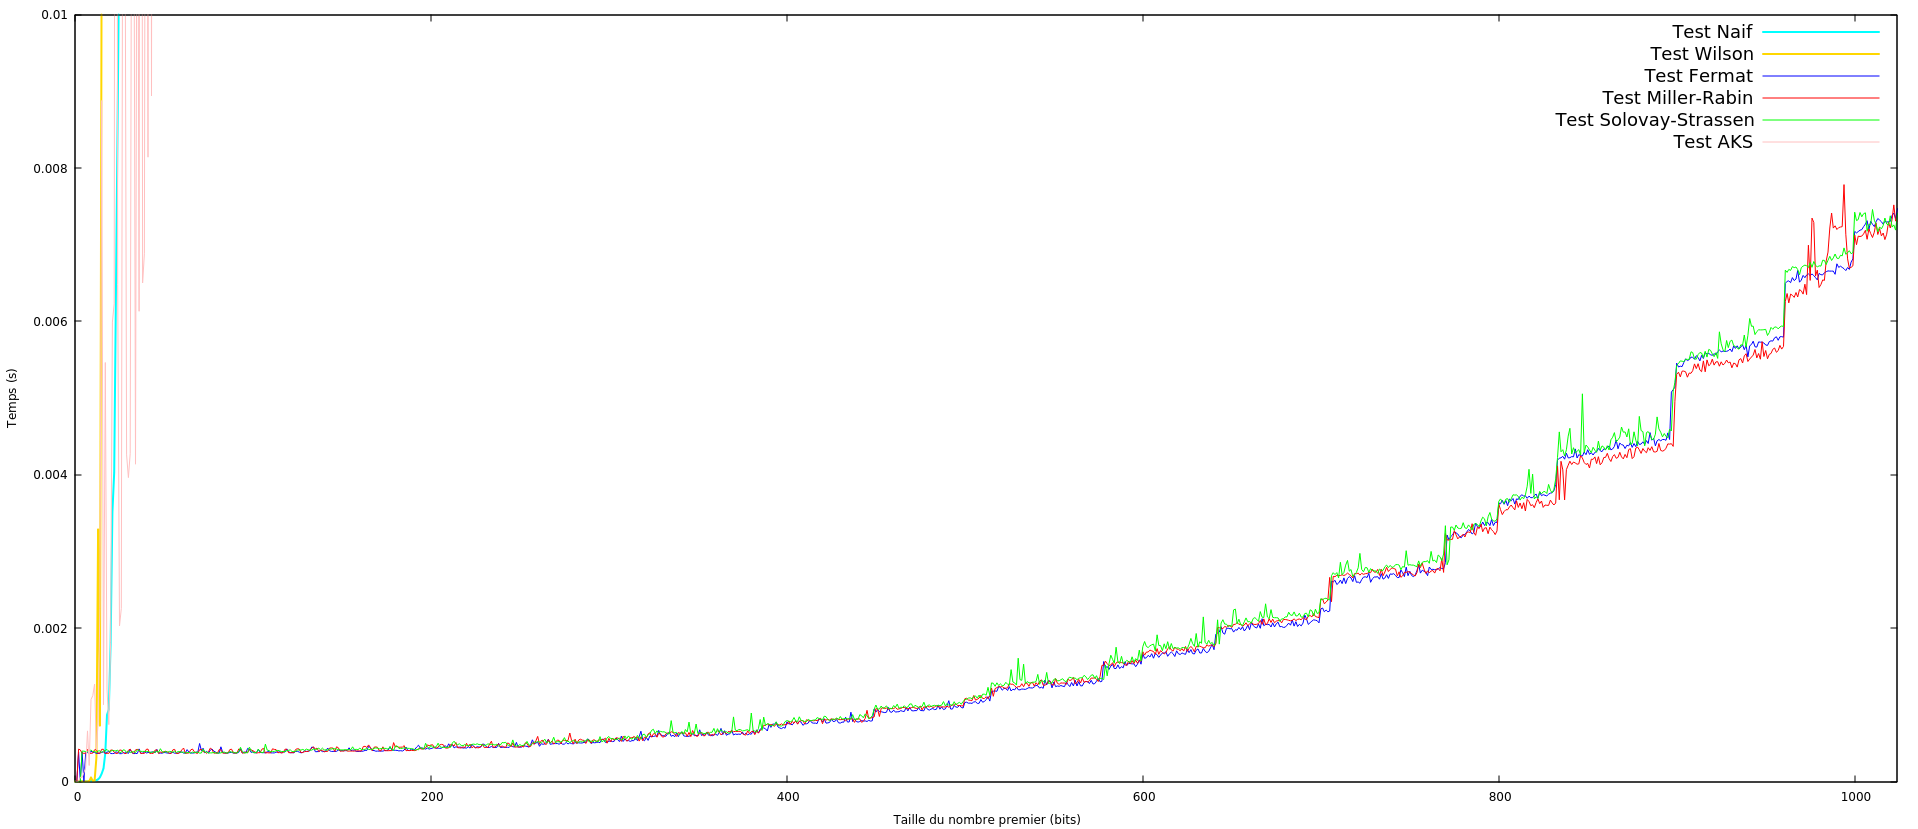
\includegraphics[width=12cm,height=7cm]{../texRapport/img/perfsAll.png}}\vspace{-1em}\caption{Temps d'exécution des tests en fonction de la taille en bits du nombre premier}\label{fig:M4}\end{figure}
		\end{frame}
		
		\begin{frame}
			\begin{figure}[H]\makebox[\textwidth]{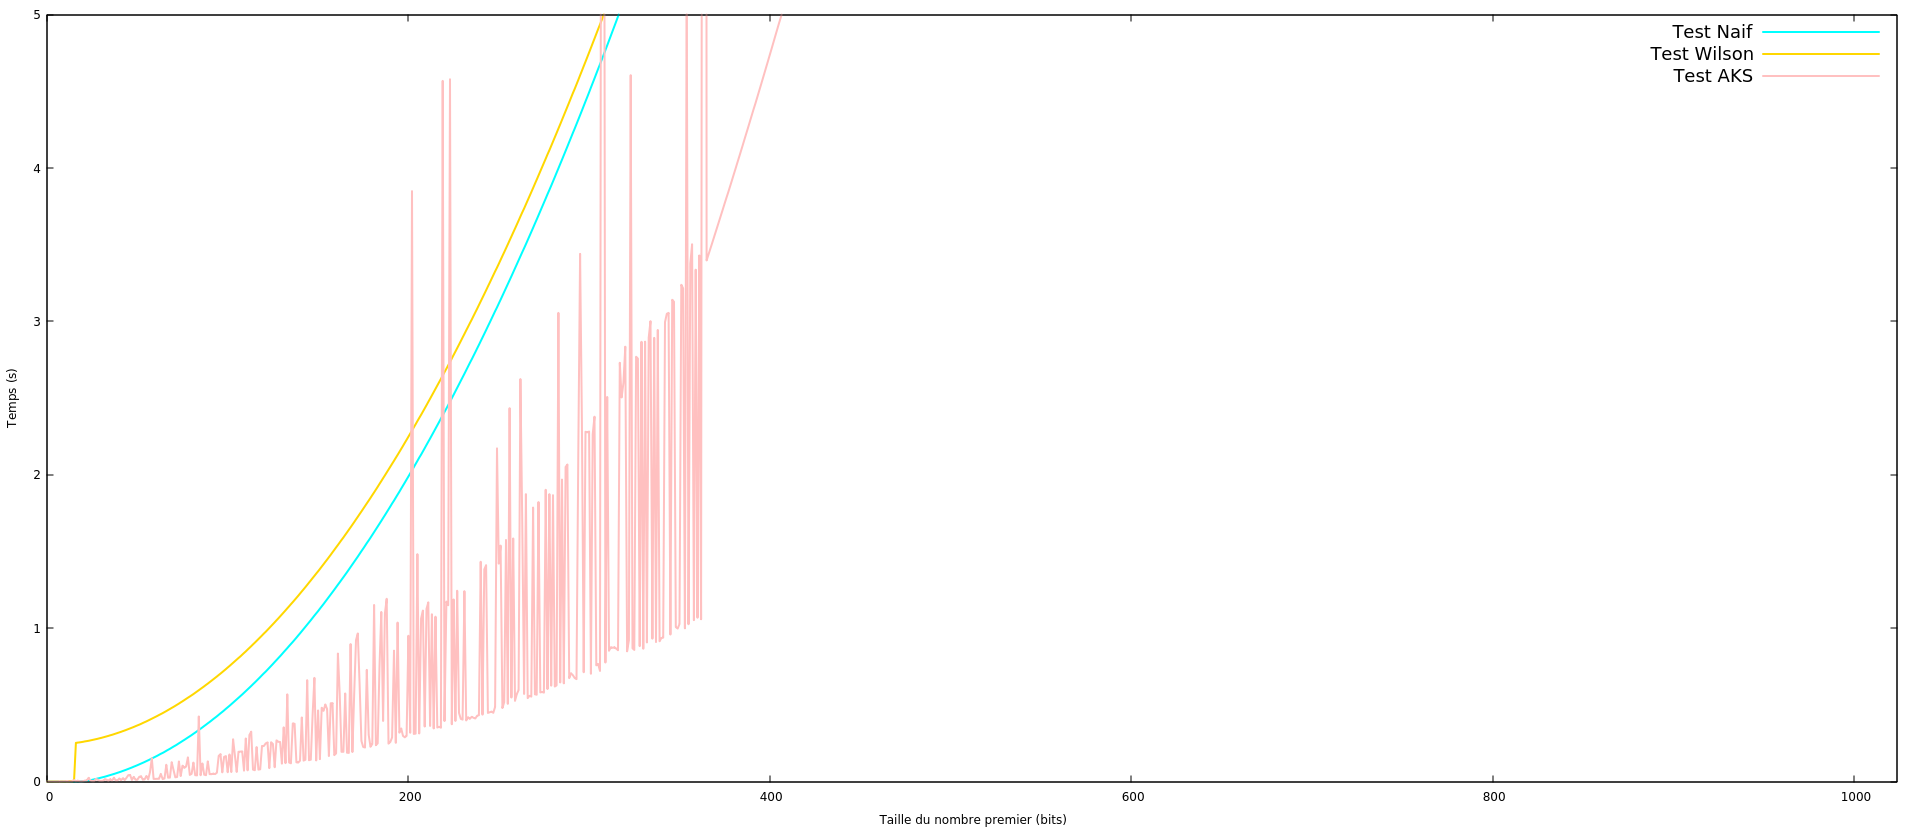
\includegraphics[width=12cm,height=7cm]{../texRapport/img/perfsDet.png}}\vspace{-1em}\caption{Temps d'exécution des tests déterministes}\label{fig:M5}\end{figure}
		\end{frame}		
		
		\begin{frame}
			\begin{figure}[H]\makebox[\textwidth]{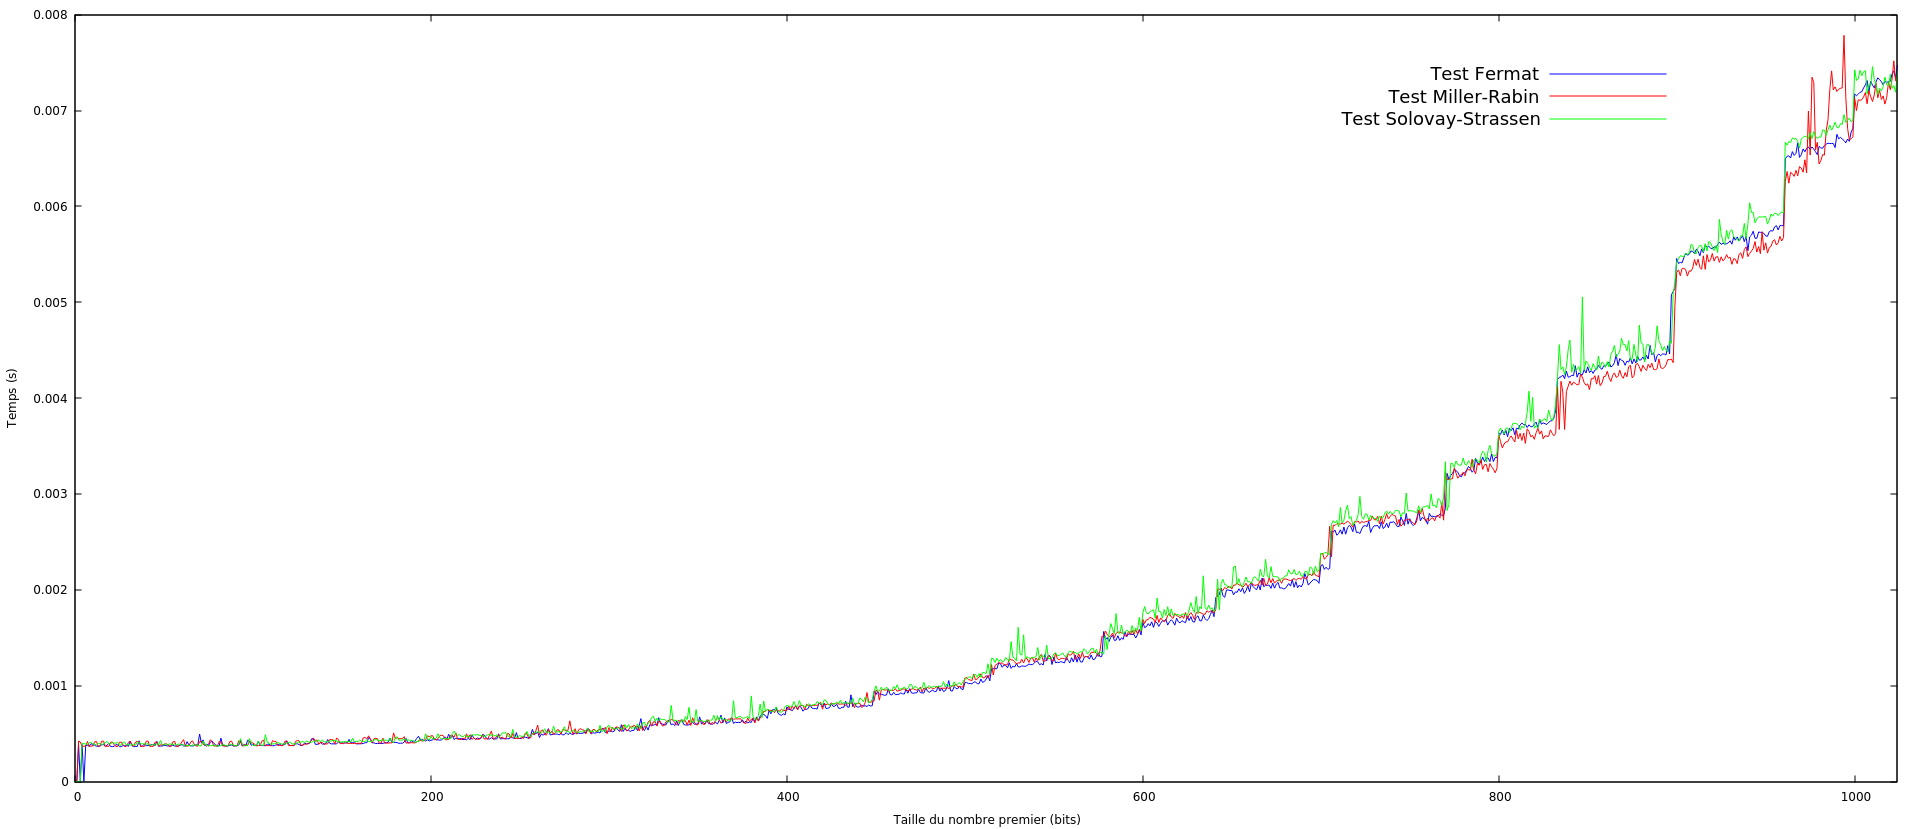
\includegraphics[width=12cm,height=7cm]{../texRapport/img/perfsProb.png}}\vspace{-1em}\caption{Temps d'exécution des tests probabilistes}\label{fig:M6}\end{figure}
		\end{frame}	
		
		\begin{frame}
			\textbf{Générateur optimal}\\~\\
			\begin{algorithm}[H]
				\caption{RPNG Optimal}\label{RPNG_opt}
				\Donnees{la taille $t$ en bits de l'entier premier à générer et le tableau tps[6][1025] des résultats de mesure du temps d'exécution des 6 test pour un nombre de bits entre 0 et 1024}
				\Sortie{un nombre premier de $t$ bits}
				Trouver le test de primalité d'indice $i$ ($i$ entre $0$ et $5$) telle que tps[i][t] est minimale (c'est-à-dire le test le plus rapide pour vérifier $t$ bits)\;
				Générer un nombre premier de $t$ bits avec le test de primalité d'indice $i$\;
			\end{algorithm}
		\end{frame}
		
	\section{Conclusion}
		\begin{frame}
			\begin{itemize}
				\item Difficultés : complexités, preuves et AKS.
				\item Améliorations : répétitions tests probabilistes
				\item Perspectives : test de primalité optimal
			\end{itemize}
		\end{frame}
	
\end{document}
